\documentclass[pdf]{beamer}
\mode<presentation>{}
\usepackage{colortbl}
\usepackage{tikz}
\usetikzlibrary{positioning}
\usetikzlibrary{arrows}
\usepackage[utf8]{inputenc}
\usepackage[T1]{fontenc}
\usepackage{mathtools}
\DeclarePairedDelimiter\ceil{\lceil}{\rceil}
\DeclarePairedDelimiter\floor{\lfloor}{\rfloor}

\setbeamertemplate{footline}[frame number]

%% preamble
\title{Tree data structures}
\author{Guillaume \textsc{Derval}}

\begin{document}

%% title frame
\begin{frame}
\titlepage
\end{frame}

{
\begin{frame}{Table of Contents}
\tableofcontents[]
\end{frame}
}

\AtBeginSection[]
{
\begin{frame}{Table of Contents}
\tableofcontents[currentsection]
\end{frame}
}

\AtBeginSubsection[]
{
\begin{frame}{Table of Contents}
\tableofcontents[currentsection, currentsubsection]
\end{frame}
}

\section{Binary Search Trees, Sets and Maps}

\begin{frame}
	\frametitle{Definition}
	A binary search tree ...
	\begin{itemize}
		\item is a tree ( :O )
		\item is binary ( :O ). So, two children maximum, that we name "left" and "right"
		\item such that each nodes stores a "key" and a "value" (which can be the same as the key)
		\item respects the "search property": 
		\begin{itemize}
			\item all nodes on the left subtree are $<$ the current node
			\item all nodes on the right subtree are $>$ the current node
		\end{itemize}
	\end{itemize}
\end{frame}

\begin{frame}
	\frametitle{Invalid BST example}
	
	\begin{center}
		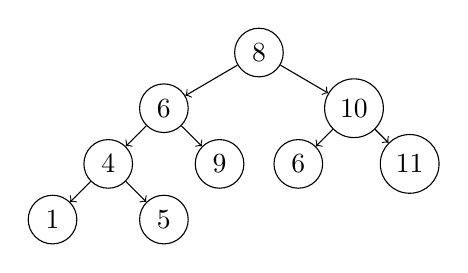
\begin{tikzpicture}[->,nodes={draw, circle}]
		\node (a8) [] {8};
		\node (a6) [below left of = a8, xshift=-0.5cm] {6};
		\node (a10) [below right of = a8, xshift=0.5cm]{10};
		\node (a4) [below left of = a6]{4};
		\node (a7) [below right of = a6]{9};
		\node (a9) [below left of = a10]{6};
		\node (a11) [below right of = a10]{11};
		\node (a1) [below left of = a4]{1};
		\node (n7) [below right of = a4]{5};
		\draw (a8) -> (a10);
		\draw (a8) -> (a6); 
		\draw (a6) -> (a4);
		\draw (a6) -> (a7);
		\draw (a10) -> (a9);
		\draw (a10) -> (a11);
		\draw (a4) -> (a1);
		\draw (a4) -> (n7);
		\end{tikzpicture}
	\end{center}
\end{frame}

\begin{frame}
	\frametitle{BST example}
	
	\begin{center}
		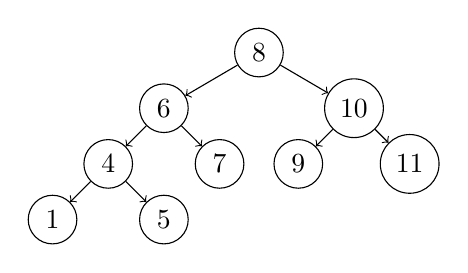
\begin{tikzpicture}[->,nodes={draw, circle}]
		\node (a8) [] {8};
		\node (a6) [below left of = a8, xshift=-0.5cm] {6};
		\node (a10) [below right of = a8, xshift=0.5cm]{10};
		\node (a4) [below left of = a6]{4};
		\node (a7) [below right of = a6]{7};
		\node (a9) [below left of = a10]{9};
		\node (a11) [below right of = a10]{11};
		\node (a1) [below left of = a4]{1};
		\node (n7) [below right of = a4]{5};
		\draw (a8) -> (a10);
		\draw (a8) -> (a6); 
		\draw (a6) -> (a4);
		\draw (a6) -> (a7);
		\draw (a10) -> (a9);
		\draw (a10) -> (a11);
		\draw (a4) -> (a1);
		\draw (a4) -> (n7);
		\end{tikzpicture}
	\end{center}
\end{frame}

\begin{frame}
	\frametitle{Balanced Search Tree}
	A (binary) tree is said to be balanced if its height is minimal, that is if its height is $\floor{\log_2(n)}$
	
	Most the of the BST are balanced. We will see later why...
\end{frame}

\begin{frame}
	\frametitle{Common operations}
	\begin{itemize}
		\item search(key): returns the value associated with the key
		\item insert(key, value): insert a new key/value
		\item findMax(): returns the key/value associated with the biggest key
		\item findMin(): ...
		\item successor(key): returns the key/value immediately after the given key
		\item predecessor(key): ...
	\end{itemize}
\end{frame}

\begin{frame}
	\frametitle{Implementing search operations}
	Let's say we want to find the value associated with $5$ in this tree:
	
	\begin{center}
		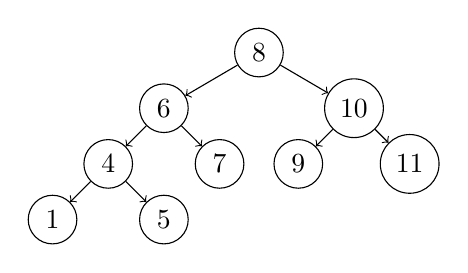
\begin{tikzpicture}[->,nodes={draw, circle}]
		\node (a8) [] {8};
		\node (a6) [below left of = a8, xshift=-0.5cm] {6};
		\node (a10) [below right of = a8, xshift=0.5cm]{10};
		\node (a4) [below left of = a6]{4};
		\node (a7) [below right of = a6]{7};
		\node (a9) [below left of = a10]{9};
		\node (a11) [below right of = a10]{11};
		\node (a1) [below left of = a4]{1};
		\node (n7) [below right of = a4]{5};
		\draw (a8) -> (a10);
		\draw (a8) -> (a6); 
		\draw (a6) -> (a4);
		\draw (a6) -> (a7);
		\draw (a10) -> (a9);
		\draw (a10) -> (a11);
		\draw (a4) -> (a1);
		\draw (a4) -> (n7);
		\end{tikzpicture}
	\end{center}
\end{frame}

\begin{frame}
	\frametitle{Implementing search operations}
	Let's start at the root:
	
	\only<2>{8 > 5: search only on the left}
	
	\begin{center}
		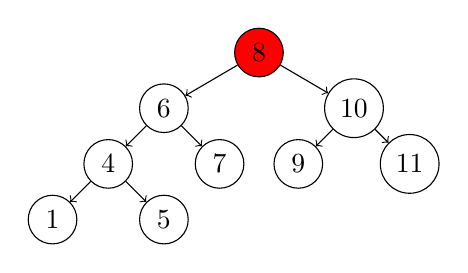
\begin{tikzpicture}[->,nodes={draw, circle}]
		\node (a8) [fill=red] {8};
		\node (a6) [below left of = a8, xshift=-0.5cm] {6};
		\node (a10) [below right of = a8, xshift=0.5cm]{10};
		\node (a4) [below left of = a6]{4};
		\node (a7) [below right of = a6]{7};
		\node (a9) [below left of = a10]{9};
		\node (a11) [below right of = a10]{11};
		\node (a1) [below left of = a4]{1};
		\node (n7) [below right of = a4]{5};
		\draw (a8) -> (a10);
		\draw (a8) -> (a6); 
		\draw (a6) -> (a4);
		\draw (a6) -> (a7);
		\draw (a10) -> (a9);
		\draw (a10) -> (a11);
		\draw (a4) -> (a1);
		\draw (a4) -> (n7);
		\end{tikzpicture}
	\end{center}
\end{frame}

\begin{frame}
	\frametitle{Implementing search operations}
	We are now at 6
	
	\only<2>{6 > 5: search only on the left}
	
	\begin{center}
		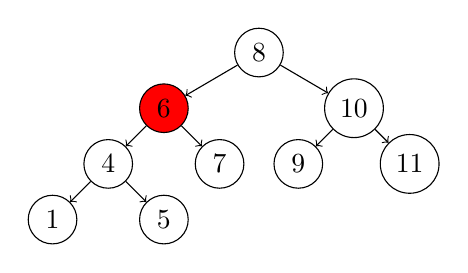
\begin{tikzpicture}[->,nodes={draw, circle}]
		\node (a8) [] {8};
		\node (a6) [below left of = a8, xshift=-0.5cm, fill=red] {6};
		\node (a10) [below right of = a8, xshift=0.5cm]{10};
		\node (a4) [below left of = a6]{4};
		\node (a7) [below right of = a6]{7};
		\node (a9) [below left of = a10]{9};
		\node (a11) [below right of = a10]{11};
		\node (a1) [below left of = a4]{1};
		\node (n7) [below right of = a4]{5};
		\draw (a8) -> (a10);
		\draw (a8) -> (a6); 
		\draw (a6) -> (a4);
		\draw (a6) -> (a7);
		\draw (a10) -> (a9);
		\draw (a10) -> (a11);
		\draw (a4) -> (a1);
		\draw (a4) -> (n7);
		\end{tikzpicture}
	\end{center}
\end{frame}

\begin{frame}
	\frametitle{Implementing search operations}
	We are now at 4
	
	\only<2>{4 < 5: search only on the right}
	
	\begin{center}
		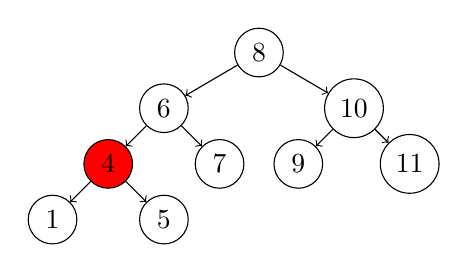
\begin{tikzpicture}[->,nodes={draw, circle}]
		\node (a8) [] {8};
		\node (a6) [below left of = a8, xshift=-0.5cm] {6};
		\node (a10) [below right of = a8, xshift=0.5cm]{10};
		\node (a4) [below left of = a6, fill=red]{4};
		\node (a7) [below right of = a6]{7};
		\node (a9) [below left of = a10]{9};
		\node (a11) [below right of = a10]{11};
		\node (a1) [below left of = a4]{1};
		\node (n7) [below right of = a4]{5};
		\draw (a8) -> (a10);
		\draw (a8) -> (a6); 
		\draw (a6) -> (a4);
		\draw (a6) -> (a7);
		\draw (a10) -> (a9);
		\draw (a10) -> (a11);
		\draw (a4) -> (a1);
		\draw (a4) -> (n7);
		\end{tikzpicture}
	\end{center}
\end{frame}

\begin{frame}
	\frametitle{Implementing search operations}
	We are now at 5. Return the key/value pair.
	
	\begin{center}
		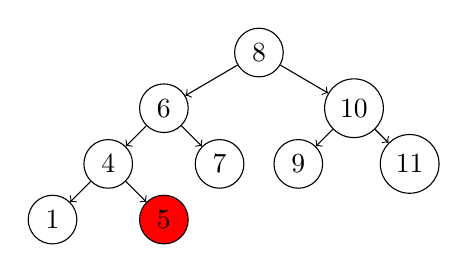
\begin{tikzpicture}[->,nodes={draw, circle}]
		\node (a8) [] {8};
		\node (a6) [below left of = a8, xshift=-0.5cm] {6};
		\node (a10) [below right of = a8, xshift=0.5cm]{10};
		\node (a4) [below left of = a6]{4};
		\node (a7) [below right of = a6]{7};
		\node (a9) [below left of = a10]{9};
		\node (a11) [below right of = a10]{11};
		\node (a1) [below left of = a4]{1};
		\node (n7) [below right of = a4, fill=red]{5};
		\draw (a8) -> (a10);
		\draw (a8) -> (a6); 
		\draw (a6) -> (a4);
		\draw (a6) -> (a7);
		\draw (a10) -> (a9);
		\draw (a10) -> (a11);
		\draw (a4) -> (a1);
		\draw (a4) -> (n7);
		\end{tikzpicture}
	\end{center}
\end{frame}

\begin{frame}
	\frametitle{Complexity?}
	\pause $O(\text{height of the tree})$
	\pause $= O(\floor{\log(n)})$ if the tree is balanced
	\vspace{2cm}
	\pause Without a balanced tree, all the operations are $O(n)$!
\end{frame}

\begin{frame}
	\frametitle{Implementing a balanced BST}
	Ideas?
\end{frame}

\begin{frame}
	\frametitle{Implementing a balanced BST}
	\begin{figure}
		\centering
		
\includegraphics[width=0.7\linewidth]{toohard}
	\end{figure}
\end{frame}

\begin{frame}
	\frametitle{Implementing a balanced BST}
	\begin{figure}
		\centering
		
\includegraphics[width=0.7\linewidth]{time}
	\end{figure}
	
	\begin{itemize}
		\pause\item Too complicated to explain right now
		\pause\item Too complicated to remember
		\pause\item Too long to implement during a contest
		\pause\item Very prone to bugs
	\end{itemize}
	Still, if you have time, it's very interesting to know, but won't be useful during competitive programming contests
\end{frame}

\begin{frame}
	\frametitle{Use the STL}
	(real) languages come with implementations of BST, in two categories
	\begin{itemize}
		\item Sets: represents a mathematical set. It is, in fact, a BST with keys==values
			\begin{itemize}
				\item C++: std::set
				\item Java: TreeSet
			\end{itemize}
		\item Maps: dictionnary
		\begin{itemize}
			\item C++: std::map
			\item Java: TreeMap
		\end{itemize}
	\end{itemize}
\end{frame}
\section{Heap}

\begin{frame}
	\frametitle{Heap}
	A heap is a structure with (mainly) two operations:
	\begin{itemize}
		\item \texttt{push}: Add an element to the heap $O(\log n)$.
		\item \texttt{pop}: remove and return the biggest/greater/... element from the heap $O(\log n)$.
	\end{itemize}
	\pause How to implement it?
	\pause With a tree, of course!
\end{frame}

\begin{frame}
	\frametitle{The heap property}
	Remember the binary search tree property?\\
	\vspace{1cm}
	\textbf{(max) Heap property}: Childrens of a node in a heap tree are $\leq$ than the node itself.\\
	\vspace{1cm}
	One of the most simple and efficient heap implementation are complete binary heap. Two more rules then:
	\begin{itemize}
		\item The tree is a binary one ($\leq$ 2 children per node)
		\item The tree is "complete": all levels of the tree are full of nodes but the last one, on which leaves are on the left
	\end{itemize}
\end{frame}


\begin{frame}
	\frametitle{Which are valid complete binary heap trees?}
	
	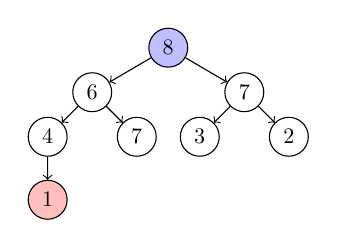
\begin{tikzpicture}[->,nodes={draw, circle,scale=0.8},scale=0.8]
	\node (a8) [fill = blue!25] {8};
	\node (a6) [below left of = a8, xshift=-0.5cm] {6};
	\node (a7) [below right of = a8, xshift=0.5cm]{7};
	\node (a4) [below left of = a6]{4};
	\node (a5) [below right of = a6]{7};
	\node (a3) [below left of = a7]{3};
	\node (a2) [below right of = a7]{2};
	\node (a1) [below of = a4, fill = red!25]{1};
	
	\draw (a8) -> (a7);
	\draw (a8) -> (a6); 
	\draw (a6) -> (a4);
	\draw (a6) -> (a5);
	\draw (a7) -> (a3);
	\draw (a7) -> (a2);
	\draw (a4) -> (a1);
	\end{tikzpicture} \only<2>{(heap property not respected on 6-7)}
	
	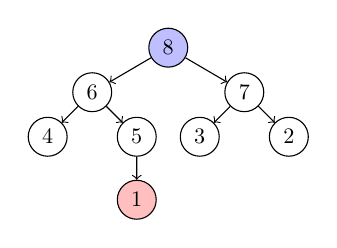
\begin{tikzpicture}[->,nodes={draw, circle,scale=0.8},scale=0.8]
	\node (a8) [fill = blue!25] {8};
	\node (a6) [below left of = a8, xshift=-0.5cm] {6};
	\node (a7) [below right of = a8, xshift=0.5cm]{7};
	\node (a4) [below left of = a6]{4};
	\node (a5) [below right of = a6]{5};
	\node (a3) [below left of = a7]{3};
	\node (a2) [below right of = a7]{2};
	\node (a1) [below of = a5, fill = red!25]{1};
	
	\draw (a8) -> (a7);
	\draw (a8) -> (a6); 
	\draw (a6) -> (a4);
	\draw (a6) -> (a5);
	\draw (a7) -> (a3);
	\draw (a7) -> (a2);
	\draw (a5) -> (a1);
	\end{tikzpicture} \only<2>{(leaf 1 not on left)}
	
	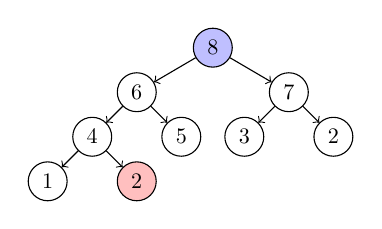
\begin{tikzpicture}[->,nodes={draw, circle,scale=0.8},scale=0.8]
	\node (a8) [fill = blue!25] {8};
	\node (a6) [below left of = a8, xshift=-0.5cm] {6};
	\node (a7) [below right of = a8, xshift=0.5cm]{7};
	\node (a4) [below left of = a6]{4};
	\node (a5) [below right of = a6]{5};
	\node (a3) [below left of = a7]{3};
	\node (a2) [below right of = a7]{2};
	\node (a1) [below left of = a4]{1};
	\node (a22) [below right of = a4, fill = red!25]{2};
	
	\draw (a8) -> (a7);
	\draw (a8) -> (a6); 
	\draw (a6) -> (a4);
	\draw (a6) -> (a5);
	\draw (a7) -> (a3);
	\draw (a7) -> (a2);
	\draw (a4) -> (a1);
	\draw (a4) -> (a22);
	\end{tikzpicture} \only<2>{(valid!)}
\end{frame}

\begin{frame}
	\frametitle{Storing a complete tree}
	Storing a complete tree is easy: use an array (or a vector)!
	\vspace{0.5cm}
	\begin{center}
		\begin{tabular}{ccccccccc}
			0 & 1 & 2 & 3 & 4 & 5 & 6 & 7 & 8\\
		\end{tabular}
		\begin{tabular}{|c|c|c|c|c|c|c|c|c|}
			\hline
			a & b & c & d & e & f & g & h & i\\
			\hline
		\end{tabular}
		
		\vspace{0.5cm}
		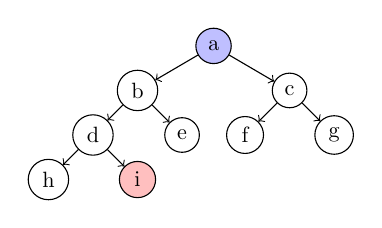
\begin{tikzpicture}[->,nodes={draw, circle,scale=0.8},scale=0.8]
		\node (a8) [fill = blue!25] {a};
		\node (a6) [below left of = a8, xshift=-0.5cm] {b};
		\node (a7) [below right of = a8, xshift=0.5cm]{c};
		\node (a4) [below left of = a6]{d};
		\node (a5) [below right of = a6]{e};
		\node (a3) [below left of = a7]{f};
		\node (a2) [below right of = a7]{g};
		\node (a1) [below left of = a4]{h};
		\node (a22) [below right of = a4, fill = red!25]{i};
		
		\draw (a8) -> (a7);
		\draw (a8) -> (a6); 
		\draw (a6) -> (a4);
		\draw (a6) -> (a5);
		\draw (a7) -> (a3);
		\draw (a7) -> (a2);
		\draw (a4) -> (a1);
		\draw (a4) -> (a22);
		\end{tikzpicture}
	\end{center}
	If $p$ is the idx of the parent in the array, idx of the children are:
	\begin{itemize}
		\item $2p+1$
		\item $2p+2$
	\end{itemize}
	Next node to be created is always at the end of the array!
\end{frame}

\begin{frame}
	\frametitle{Adding a new element}
	\begin{enumerate}
		\item Add new element at the end of the tree
		\item If parent does not respect the heap property (== is lesser than the new node)
		\begin{enumerate}
			\item Exchange the node and its parent
			\item Repeat from 2.
		\end{enumerate}
	\end{enumerate}
\end{frame}

\begin{frame}
	\frametitle{Adding a new element}
	Adding $7$:
	\begin{center}
	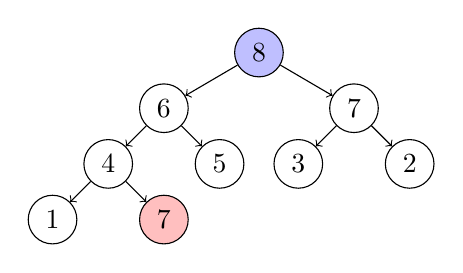
\begin{tikzpicture}[->,nodes={draw, circle}]
	\node (a8) [fill = blue!25] {8};
	\node (a6) [below left of = a8, xshift=-0.5cm] {6};
	\node (a7) [below right of = a8, xshift=0.5cm]{7};
	\node (a4) [below left of = a6]{4};
	\node (a5) [below right of = a6]{5};
	\node (a3) [below left of = a7]{3};
	\node (a2) [below right of = a7]{2};
	\node (a1) [below left of = a4]{1};
	\node (n7) [below right of = a4, fill = red!25]{7};
	\draw (a8) -> (a7);
	\draw (a8) -> (a6); 
	\draw (a6) -> (a4);
	\draw (a6) -> (a5);
	\draw (a7) -> (a3);
	\draw (a7) -> (a2);
	\draw (a4) -> (a1);
	\draw (a4) -> (n7);
	\end{tikzpicture}
	\end{center}
\end{frame}

\begin{frame}
	\frametitle{Adding a new element}
	Adding $7$:
	\begin{center}
		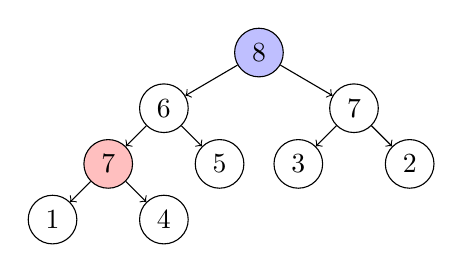
\begin{tikzpicture}[->,nodes={draw, circle}]
		\node (a8) [fill = blue!25] {8};
		\node (a6) [below left of = a8, xshift=-0.5cm] {6};
		\node (a7) [below right of = a8, xshift=0.5cm]{7};
		\node (a4) [below left of = a6, fill = red!25]{7};
		\node (a5) [below right of = a6]{5};
		\node (a3) [below left of = a7]{3};
		\node (a2) [below right of = a7]{2};
		\node (a1) [below left of = a4]{1};
		\node (n7) [below right of = a4]{4};
		\draw (a8) -> (a7);
		\draw (a8) -> (a6); 
		\draw (a6) -> (a4);
		\draw (a6) -> (a5);
		\draw (a7) -> (a3);
		\draw (a7) -> (a2);
		\draw (a4) -> (a1);
		\draw (a4) -> (n7);
		\end{tikzpicture}
	\end{center}
\end{frame}

\begin{frame}
	\frametitle{Adding a new element}
	Adding $7$:
	\begin{center}
		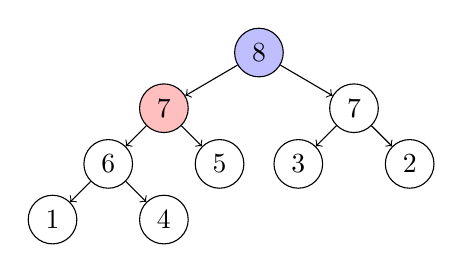
\begin{tikzpicture}[->,nodes={draw, circle}]
		\node (a8) [fill = blue!25] {8};
		\node (a6) [below left of = a8, xshift=-0.5cm, fill = red!25] {7};
		\node (a7) [below right of = a8, xshift=0.5cm]{7};
		\node (a4) [below left of = a6]{6};
		\node (a5) [below right of = a6]{5};
		\node (a3) [below left of = a7]{3};
		\node (a2) [below right of = a7]{2};
		\node (a1) [below left of = a4]{1};
		\node (n7) [below right of = a4]{4};
		\draw (a8) -> (a7);
		\draw (a8) -> (a6); 
		\draw (a6) -> (a4);
		\draw (a6) -> (a5);
		\draw (a7) -> (a3);
		\draw (a7) -> (a2);
		\draw (a4) -> (a1);
		\draw (a4) -> (n7);
		\end{tikzpicture}
	\end{center}
\end{frame}

\begin{frame}
	\frametitle{Adding a new element}
	Adding $7$:
	\begin{center}
		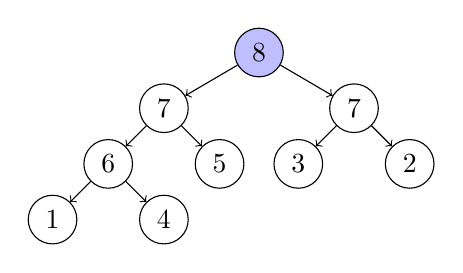
\begin{tikzpicture}[->,nodes={draw, circle}]
		\node (a8) [fill = blue!25] {8};
		\node (a6) [below left of = a8, xshift=-0.5cm] {7};
		\node (a7) [below right of = a8, xshift=0.5cm]{7};
		\node (a4) [below left of = a6]{6};
		\node (a5) [below right of = a6]{5};
		\node (a3) [below left of = a7]{3};
		\node (a2) [below right of = a7]{2};
		\node (a1) [below left of = a4]{1};
		\node (n7) [below right of = a4]{4};
		\draw (a8) -> (a7);
		\draw (a8) -> (a6); 
		\draw (a6) -> (a4);
		\draw (a6) -> (a5);
		\draw (a7) -> (a3);
		\draw (a7) -> (a2);
		\draw (a4) -> (a1);
		\draw (a4) -> (n7);
		\end{tikzpicture}
	\end{center}
\end{frame}

\begin{frame}
	\frametitle{Removing the first element}
	\begin{enumerate}
		\item Save somewhere the root of the tree to return it later
		\item Take the last node value, and put it at the top of the tree
		\item Three cases then:
			\begin{itemize}
				\item If the heap property is respected (node $\geq$ its children), return
				\item If one of the children is $>$ the node, swap them and repeat from 3.
				\item If both children are $>$ the node, swap with the greatest child and repeat from 3.
			\end{itemize}
	\end{enumerate}
\end{frame}

\begin{frame}
	\frametitle{Removing the first element}
	Step 1: store the root somewhere (remember: root was 8)
	
	\begin{center}
		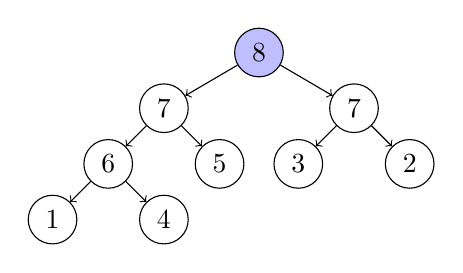
\begin{tikzpicture}[->,nodes={draw, circle}]
		\node (a8) [fill = blue!25] {8};
		\node (a6) [below left of = a8, xshift=-0.5cm] {7};
		\node (a7) [below right of = a8, xshift=0.5cm]{7};
		\node (a4) [below left of = a6]{6};
		\node (a5) [below right of = a6]{5};
		\node (a3) [below left of = a7]{3};
		\node (a2) [below right of = a7]{2};
		\node (a1) [below left of = a4]{1};
		\node (n7) [below right of = a4]{4};
		\draw (a8) -> (a7);
		\draw (a8) -> (a6); 
		\draw (a6) -> (a4);
		\draw (a6) -> (a5);
		\draw (a7) -> (a3);
		\draw (a7) -> (a2);
		\draw (a4) -> (a1);
		\draw (a4) -> (n7);
		\end{tikzpicture}
	\end{center}
\end{frame}

\begin{frame}
	\frametitle{Removing the first element}
	Step 2: put the last node at the root
	
	\begin{center}
		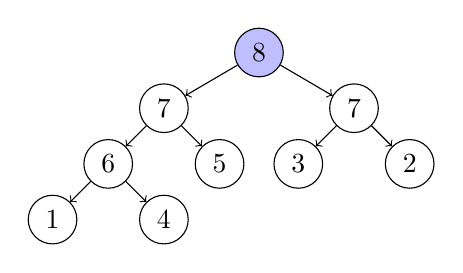
\begin{tikzpicture}[->,nodes={draw, circle}]
		\node (a8) [fill = blue!25] {8};
		\node (a6) [below left of = a8, xshift=-0.5cm] {7};
		\node (a7) [below right of = a8, xshift=0.5cm]{7};
		\node (a4) [below left of = a6]{6};
		\node (a5) [below right of = a6]{5};
		\node (a3) [below left of = a7]{3};
		\node (a2) [below right of = a7]{2};
		\node (a1) [below left of = a4]{1};
		\node (n7) [below right of = a4]{4};
		\draw (a8) -> (a7);
		\draw (a8) -> (a6); 
		\draw (a6) -> (a4);
		\draw (a6) -> (a5);
		\draw (a7) -> (a3);
		\draw (a7) -> (a2);
		\draw (a4) -> (a1);
		\draw (a4) -> (n7);
		\end{tikzpicture}
	\end{center}
\end{frame}

\begin{frame}
	\frametitle{Removing the first element}
	Step 2: put the last node at the root
	
	\begin{center}
		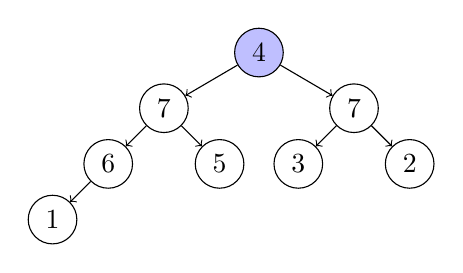
\begin{tikzpicture}[->,nodes={draw, circle}]
		\node (a8) [fill = blue!25] {4};
		\node (a6) [below left of = a8, xshift=-0.5cm] {7};
		\node (a7) [below right of = a8, xshift=0.5cm]{7};
		\node (a4) [below left of = a6]{6};
		\node (a5) [below right of = a6]{5};
		\node (a3) [below left of = a7]{3};
		\node (a2) [below right of = a7]{2};
		\node (a1) [below left of = a4]{1};
		\draw (a8) -> (a7);
		\draw (a8) -> (a6); 
		\draw (a6) -> (a4);
		\draw (a6) -> (a5);
		\draw (a7) -> (a3);
		\draw (a7) -> (a2);
		\draw (a4) -> (a1);
		\end{tikzpicture}
	\end{center}
\end{frame}

\begin{frame}
	\frametitle{Removing the first element}
	Step 3: check heap property with the children of the node.\\
	\only<2>{\textbf{Not respected -> swap with (the first) 7}}
	\begin{center}
		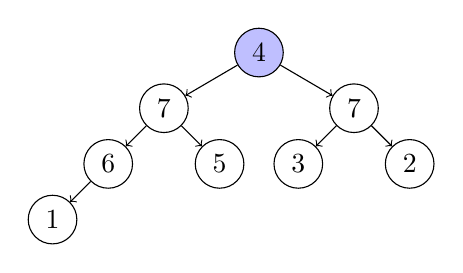
\begin{tikzpicture}[->,nodes={draw, circle}]
		\node (a8) [fill = blue!25] {4};
		\node (a6) [below left of = a8, xshift=-0.5cm] {7};
		\node (a7) [below right of = a8, xshift=0.5cm]{7};
		\node (a4) [below left of = a6]{6};
		\node (a5) [below right of = a6]{5};
		\node (a3) [below left of = a7]{3};
		\node (a2) [below right of = a7]{2};
		\node (a1) [below left of = a4]{1};
		\draw (a8) -> (a7);
		\draw (a8) -> (a6); 
		\draw (a6) -> (a4);
		\draw (a6) -> (a5);
		\draw (a7) -> (a3);
		\draw (a7) -> (a2);
		\draw (a4) -> (a1);
		\end{tikzpicture}
	\end{center}
\end{frame}

\begin{frame}
	\frametitle{Removing the first element}
	Step 3: check heap property with the children of the node.\\
	\textbf{Not respected -> swap with (the first) 7}
	\begin{center}
		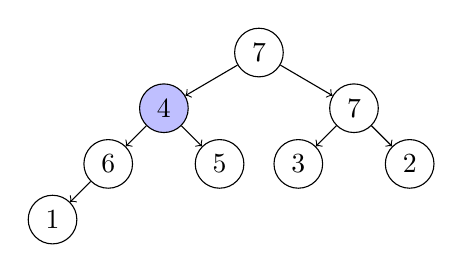
\begin{tikzpicture}[->,nodes={draw, circle}]
		\node (a8) [] {7};
		\node (a6) [below left of = a8, xshift=-0.5cm,fill = blue!25] {4};
		\node (a7) [below right of = a8, xshift=0.5cm]{7};
		\node (a4) [below left of = a6]{6};
		\node (a5) [below right of = a6]{5};
		\node (a3) [below left of = a7]{3};
		\node (a2) [below right of = a7]{2};
		\node (a1) [below left of = a4]{1};
		\draw (a8) -> (a7);
		\draw (a8) -> (a6); 
		\draw (a6) -> (a4);
		\draw (a6) -> (a5);
		\draw (a7) -> (a3);
		\draw (a7) -> (a2);
		\draw (a4) -> (a1);
		\end{tikzpicture}
	\end{center}
\end{frame}

\begin{frame}
	\frametitle{Removing the first element}
	Step 3: check heap property with the children of the node.\\
	\textbf{Not respected -> swap with 6 (the greatest child)}
	\begin{center}
		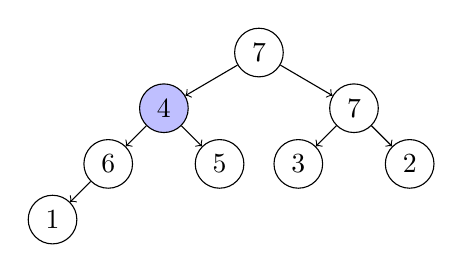
\begin{tikzpicture}[->,nodes={draw, circle}]
		\node (a8) [] {7};
		\node (a6) [below left of = a8, xshift=-0.5cm,fill = blue!25] {4};
		\node (a7) [below right of = a8, xshift=0.5cm]{7};
		\node (a4) [below left of = a6]{6};
		\node (a5) [below right of = a6]{5};
		\node (a3) [below left of = a7]{3};
		\node (a2) [below right of = a7]{2};
		\node (a1) [below left of = a4]{1};
		\draw (a8) -> (a7);
		\draw (a8) -> (a6); 
		\draw (a6) -> (a4);
		\draw (a6) -> (a5);
		\draw (a7) -> (a3);
		\draw (a7) -> (a2);
		\draw (a4) -> (a1);
		\end{tikzpicture}
	\end{center}
\end{frame}

\begin{frame}
	\frametitle{Removing the first element}
	Step 3: check heap property with the children of the node.\\
	\textbf{Not respected -> swap with 6 (the greatest child)}
	\begin{center}
		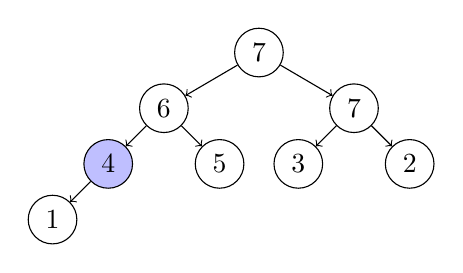
\begin{tikzpicture}[->,nodes={draw, circle}]
		\node (a8) [] {7};
		\node (a6) [below left of = a8, xshift=-0.5cm] {6};
		\node (a7) [below right of = a8, xshift=0.5cm]{7};
		\node (a4) [below left of = a6,fill = blue!25]{4};
		\node (a5) [below right of = a6]{5};
		\node (a3) [below left of = a7]{3};
		\node (a2) [below right of = a7]{2};
		\node (a1) [below left of = a4]{1};
		\draw (a8) -> (a7);
		\draw (a8) -> (a6); 
		\draw (a6) -> (a4);
		\draw (a6) -> (a5);
		\draw (a7) -> (a3);
		\draw (a7) -> (a2);
		\draw (a4) -> (a1);
		\end{tikzpicture}
	\end{center}
\end{frame}

\begin{frame}
	\frametitle{Removing the first element}
	Step 3: check heap property with the children of the node.\\
	\textbf{Done}
	\begin{center}
		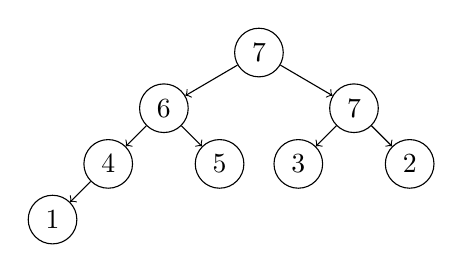
\begin{tikzpicture}[->,nodes={draw, circle}]
		\node (a8) [] {7};
		\node (a6) [below left of = a8, xshift=-0.5cm] {6};
		\node (a7) [below right of = a8, xshift=0.5cm]{7};
		\node (a4) [below left of = a6]{4};
		\node (a5) [below right of = a6]{5};
		\node (a3) [below left of = a7]{3};
		\node (a2) [below right of = a7]{2};
		\node (a1) [below left of = a4]{1};
		\draw (a8) -> (a7);
		\draw (a8) -> (a6); 
		\draw (a6) -> (a4);
		\draw (a6) -> (a5);
		\draw (a7) -> (a3);
		\draw (a7) -> (a2);
		\draw (a4) -> (a1);
		\end{tikzpicture}
	\end{center}
\end{frame}

\begin{frame}
	\frametitle{Usage}
	\begin{itemize}
		\item Priority queues
		\item Dijkstra
		\item Sorting
		\item ...
	\end{itemize}
	
	\begin{itemize}
		\item In C++: std::priority\_queue
		\item In Java: PriorityQueue
	\end{itemize}
\end{frame}
%\section{Problem set}

\subsection{Mixtures}

Harry Potter has $n$ mixtures in front of him, arranged in a row.
Each mixture has one of 100 different colors (colors have numbers from 0 to 99).

He wants to mix all these mixtures together.
At each step, he is going to take two mixtures that stand next to each other
and mix them together, and put the resulting mixture in their place.

When mixing two mixtures of colors $a$ and $b$,
the resulting mixture will have the color $(a+b) \mod 100$.

Also, there will be some smoke in the process.
The amount of smoke generated when mixing
two mixtures of colors $a$ and $b$ is $a\times b$.

Find out what is the minimum amount of smoke that Harry can get when mixing all the ixtures together.

\subsubsection*{Input}
There will be a number of test cases in the input.

The first line of each test case will contain $n$, the number of mixtures,
$1 \leq n \leq 100$.

The second line will contain n integers between 0 and 99
--- the initial colors of the mixtures.

\subsubsection*{Output}
For each test case, output the minimum amount of smoke.

\subsubsection*{Limits}
\begin{itemize}
    \item Time limit: 9\,sec
    \item Memory limit: 256\,MB
\end{itemize}



\subsubsection*{Example}
\begin{verbatim}
Input:
2
18 19
3
40 60 20
Output:
342
2400
\end{verbatim}

\subsubsection*{Notes}
In the second test case, there are two possibilities:
\begin{itemize}
    \item first mix 40 and 60 (smoke: 2400), getting 0,
        then mix 0 and 20 (smoke: 0); total amount of smoke is 2400
    \item first mix 60 and 20 (smoke: 1200), getting 80,
        then mix 40 and 80 (smoke: 3200);
        total amount of smoke is 4400
\end{itemize}

The first scenario is the correct approach since
it minimizes the amount of smoke produced.

\subsubsection*{Source} \url{http://www.codechef.com/problems/MIXTURES}

\subsection{Fox and Number Game}

Fox Ciel is playing a game with numbers now.

Ciel has $n$ positive integers: $x_1,x_2,\ldots,x_n$.
She can do the following operation as many times as needed:
select two different indexes $i$ and $j$ such that $x_i>x_j$ holds,
and then apply assignment $x_i = x_i - x_j$.
The goal is to make the sum of all numbers as small as possible.

Please help Ciel find this minimal sum.

\subsubsection*{Input}
The first line contains an integer $n$ ($2 \leq n \leq 100).$
Then the second line contains $n$ integers: $x_1,x_2,\ldots,x_n$
($1\leq x_i \leq 100$).

\subsubsection*{Output}
Output a single integer --- the required minimal sum.

\subsubsection*{Limits}
\begin{itemize}
    \item Time limit: 1\,sec
    \item Memory limit: 256\,MB
\end{itemize}



\subsubsection*{Examples}
\begin{verbatim}
Input:
2
1 2
Output:
2

Input:
3
2 4 6
Output:
6

Input:
2
12 18
Output:
12

Input:
5
45 12 27 30 18
Output:
15
\end{verbatim}

\subsubsection*{Notes}
In the first example the optimal way is to do the assignment
$x_2 = x_2 - x_1$.

In the second example the optimal sequence of operations is:
$x_3 = x_3-x_2$, $x_2 = x_2-x_1$.

\subsection*{Source} \url{http://codeforces.com/problemset/problem/389/A}

\subsection{George and Number}

George is a cat, so he really likes to play.
Most of all he likes to play with his array of positive integers b.
During the game, George modifies the array by using special changes.
Let's mark George's current array as $b_1,b_2,\ldots,b_{|b|}$
(record $|b|$ denotes the current length of the array).
Then one change is a sequence of actions: 
\begin{itemize}
    \item Choose two distinct indexes $i$ and $j$
        ($1\leq i,j \leq |b|,\ i \neq j$), such that $b_i \geq b_j$.
    \item Get number $v$ = concat$(b_i,b_j)$,
        where concat$(x,y)$ is a number obtained by adding number $y$
        to the end of the decimal record of number $x$.
        For example, concat$(500,10)=50010$, concat$(2,2)=22$.
    \item Add number $v$ to the end of the array.
        The length of the array will increase by one.
    \item Remove from the array numbers with indexes $i$ and $j$.
        The length of the array will decrease by two,
        and elements of the array will become re-numbered
        from 1 to current length of the array.
\end{itemize}
George played for a long time with his array $b$ and received from array $b$
an array consisting of exactly one number $p$.
Now George wants to know: what is the maximum number of elements array $b$
could contain originally?
Help him find this number.
Note that originally the array could contain only \emph{positive} integers.

\subsubsection*{Input}
The first line of the input contains a single integer $p$
($1 \leq p < 10^{100000}$).
It is guaranteed that number $p$ doesn't contain any leading zeroes.

\subsubsection*{Output}
Print an integer --- the maximum number of elements array $b$
could contain originally.

\subsubsection*{Limits}
\begin{itemize}
    \item Time limit: 1\,sec
    \item Memory limit: 256\,MB
\end{itemize}

\subsubsection*{Examples}
\begin{verbatim}
Input:
9555
Output:
4

Input:
10000000005
Output:
2

Input:
800101
Output:
3

Input:
45
Output:
1

Input:
1000000000000001223300003342220044555
Output:
17

Input:
19992000
Output:
1

Input:
310200
Output:
2
\end{verbatim}

\subsubsection*{Notes}
Let's consider the test examples:
\begin{itemize}
    \item Originally array b can be equal to $\{5,9,5,5\}$.
        The sequence of George's changes could have been:
        $\{5,9,5,5\}\rightarrow\{5,5,95\}\rightarrow\{95,55\}
        \rightarrow\{9555\}$.
    \item Originally array $b$ could be equal to $\{1000000000,5\}$.
        Please note that the array $b$ cannot contain zeros.
    \item Originally array $b$ could be equal to $\{800,10,1\}$.
    \item Originally array $b$ could be equal to $\{45\}$.
        It cannot be equal to $\{4,5\}$,
        because George can get only array $\{45\}$ from this array
        in one operation.
\end{itemize}
Note that the numbers can be very large.

\subsubsection*{Source} \url{http://codeforces.com/problemset/problem/387/C}

\subsection{Bytelandian gold coins}

In Byteland they have a very strange monetary system.

Each Bytelandian gold coin has an integer number written on it. A coin $n$
can be exchanged in a bank into three coins: $n/2$, $n/3$ and $n/4$.
But these numbers are all rounded down (the banks have to make a profit).

You can also sell Bytelandian coins for American dollars. The exchange
rate is $1:1$. But you can not buy Bytelandian coins.

You have one gold coin. What is the maximum amount of American dollars
you can get for it?

\subsubsection*{Input}
The input will contain several test cases (not more than 10). Each
testcase is a single line with a number $n$, $0 \leq n \leq 1\,000\,000\,000$.
It is the number written on your coin.

\subsubsection*{Output}
For each test case output a single line, containing the maximum amount
of American dollars you can make.

\subsubsection*{Limits}
\begin{itemize}
    \item Time limit: 9\,sec
    \item Memory limit: 256\,MB
\end{itemize}



\subsubsection*{Example}
\begin{verbatim}
Input:
12
2
Output:
13
2
\end{verbatim}

\subsubsection*{Notes}
You can change 12 into 6, 4 and 3, and then change these into
$\$6+\$4+\$3 = \$13$.

If you try changing the coin 2 into 3 smaller coins, you will get
1, 0 and 0, and later you can get no more than \$1 out of them.
It is better just to change the 2 coin directly into \$2.

\subsubsection*{Source} \url{http://www.codechef.com/problems/COINS}


%\section{Problem set}

\subsection{Mixtures}

Harry Potter has $n$ mixtures in front of him, arranged in a row.
Each mixture has one of 100 different colors (colors have numbers from 0 to 99).

He wants to mix all these mixtures together.
At each step, he is going to take two mixtures that stand next to each other
and mix them together, and put the resulting mixture in their place.

When mixing two mixtures of colors $a$ and $b$,
the resulting mixture will have the color $(a+b) \mod 100$.

Also, there will be some smoke in the process.
The amount of smoke generated when mixing
two mixtures of colors $a$ and $b$ is $a\times b$.

Find out what is the minimum amount of smoke that Harry can get when mixing all the ixtures together.

\subsubsection*{Input}
There will be a number of test cases in the input.

The first line of each test case will contain $n$, the number of mixtures,
$1 \leq n \leq 100$.

The second line will contain n integers between 0 and 99
--- the initial colors of the mixtures.

\subsubsection*{Output}
For each test case, output the minimum amount of smoke.

\subsubsection*{Limits}
\begin{itemize}
    \item Time limit: 9\,sec
    \item Memory limit: 256\,MB
\end{itemize}



\subsubsection*{Example}
\begin{verbatim}
Input:
2
18 19
3
40 60 20
Output:
342
2400
\end{verbatim}

\subsubsection*{Notes}
In the second test case, there are two possibilities:
\begin{itemize}
    \item first mix 40 and 60 (smoke: 2400), getting 0,
        then mix 0 and 20 (smoke: 0); total amount of smoke is 2400
    \item first mix 60 and 20 (smoke: 1200), getting 80,
        then mix 40 and 80 (smoke: 3200);
        total amount of smoke is 4400
\end{itemize}

The first scenario is the correct approach since
it minimizes the amount of smoke produced.

\subsubsection*{Source} \url{http://www.codechef.com/problems/MIXTURES}

\subsection{Fox and Number Game}

Fox Ciel is playing a game with numbers now.

Ciel has $n$ positive integers: $x_1,x_2,\ldots,x_n$.
She can do the following operation as many times as needed:
select two different indexes $i$ and $j$ such that $x_i>x_j$ holds,
and then apply assignment $x_i = x_i - x_j$.
The goal is to make the sum of all numbers as small as possible.

Please help Ciel find this minimal sum.

\subsubsection*{Input}
The first line contains an integer $n$ ($2 \leq n \leq 100).$
Then the second line contains $n$ integers: $x_1,x_2,\ldots,x_n$
($1\leq x_i \leq 100$).

\subsubsection*{Output}
Output a single integer --- the required minimal sum.

\subsubsection*{Limits}
\begin{itemize}
    \item Time limit: 1\,sec
    \item Memory limit: 256\,MB
\end{itemize}



\subsubsection*{Examples}
\begin{verbatim}
Input:
2
1 2
Output:
2

Input:
3
2 4 6
Output:
6

Input:
2
12 18
Output:
12

Input:
5
45 12 27 30 18
Output:
15
\end{verbatim}

\subsubsection*{Notes}
In the first example the optimal way is to do the assignment
$x_2 = x_2 - x_1$.

In the second example the optimal sequence of operations is:
$x_3 = x_3-x_2$, $x_2 = x_2-x_1$.

\subsection*{Source} \url{http://codeforces.com/problemset/problem/389/A}

\subsection{George and Number}

George is a cat, so he really likes to play.
Most of all he likes to play with his array of positive integers b.
During the game, George modifies the array by using special changes.
Let's mark George's current array as $b_1,b_2,\ldots,b_{|b|}$
(record $|b|$ denotes the current length of the array).
Then one change is a sequence of actions: 
\begin{itemize}
    \item Choose two distinct indexes $i$ and $j$
        ($1\leq i,j \leq |b|,\ i \neq j$), such that $b_i \geq b_j$.
    \item Get number $v$ = concat$(b_i,b_j)$,
        where concat$(x,y)$ is a number obtained by adding number $y$
        to the end of the decimal record of number $x$.
        For example, concat$(500,10)=50010$, concat$(2,2)=22$.
    \item Add number $v$ to the end of the array.
        The length of the array will increase by one.
    \item Remove from the array numbers with indexes $i$ and $j$.
        The length of the array will decrease by two,
        and elements of the array will become re-numbered
        from 1 to current length of the array.
\end{itemize}
George played for a long time with his array $b$ and received from array $b$
an array consisting of exactly one number $p$.
Now George wants to know: what is the maximum number of elements array $b$
could contain originally?
Help him find this number.
Note that originally the array could contain only \emph{positive} integers.

\subsubsection*{Input}
The first line of the input contains a single integer $p$
($1 \leq p < 10^{100000}$).
It is guaranteed that number $p$ doesn't contain any leading zeroes.

\subsubsection*{Output}
Print an integer --- the maximum number of elements array $b$
could contain originally.

\subsubsection*{Limits}
\begin{itemize}
    \item Time limit: 1\,sec
    \item Memory limit: 256\,MB
\end{itemize}

\subsubsection*{Examples}
\begin{verbatim}
Input:
9555
Output:
4

Input:
10000000005
Output:
2

Input:
800101
Output:
3

Input:
45
Output:
1

Input:
1000000000000001223300003342220044555
Output:
17

Input:
19992000
Output:
1

Input:
310200
Output:
2
\end{verbatim}

\subsubsection*{Notes}
Let's consider the test examples:
\begin{itemize}
    \item Originally array b can be equal to $\{5,9,5,5\}$.
        The sequence of George's changes could have been:
        $\{5,9,5,5\}\rightarrow\{5,5,95\}\rightarrow\{95,55\}
        \rightarrow\{9555\}$.
    \item Originally array $b$ could be equal to $\{1000000000,5\}$.
        Please note that the array $b$ cannot contain zeros.
    \item Originally array $b$ could be equal to $\{800,10,1\}$.
    \item Originally array $b$ could be equal to $\{45\}$.
        It cannot be equal to $\{4,5\}$,
        because George can get only array $\{45\}$ from this array
        in one operation.
\end{itemize}
Note that the numbers can be very large.

\subsubsection*{Source} \url{http://codeforces.com/problemset/problem/387/C}

\subsection{Bytelandian gold coins}

In Byteland they have a very strange monetary system.

Each Bytelandian gold coin has an integer number written on it. A coin $n$
can be exchanged in a bank into three coins: $n/2$, $n/3$ and $n/4$.
But these numbers are all rounded down (the banks have to make a profit).

You can also sell Bytelandian coins for American dollars. The exchange
rate is $1:1$. But you can not buy Bytelandian coins.

You have one gold coin. What is the maximum amount of American dollars
you can get for it?

\subsubsection*{Input}
The input will contain several test cases (not more than 10). Each
testcase is a single line with a number $n$, $0 \leq n \leq 1\,000\,000\,000$.
It is the number written on your coin.

\subsubsection*{Output}
For each test case output a single line, containing the maximum amount
of American dollars you can make.

\subsubsection*{Limits}
\begin{itemize}
    \item Time limit: 9\,sec
    \item Memory limit: 256\,MB
\end{itemize}



\subsubsection*{Example}
\begin{verbatim}
Input:
12
2
Output:
13
2
\end{verbatim}

\subsubsection*{Notes}
You can change 12 into 6, 4 and 3, and then change these into
$\$6+\$4+\$3 = \$13$.

If you try changing the coin 2 into 3 smaller coins, you will get
1, 0 and 0, and later you can get no more than \$1 out of them.
It is better just to change the 2 coin directly into \$2.

\subsubsection*{Source} \url{http://www.codechef.com/problems/COINS}



\end{document}